%!TEX TS-program = xelatex

%%%%%%%%%%%%%%%%%%%%%%%%%%%%%%%%%%%%%%%%%%%%%%%%
% CV template
% Originally created by Adrien Friggeri
% Improved by Carmine Benedetto
%%%%%%%%%%%%%%%%%%%%%%%%%%%%%%%%%%%%%%%%%%%%%%%%

\documentclass[]{cv-class}
\usepackage{afterpage}
\usepackage{hyperref}
\usepackage{color}
\usepackage{xcolor}
\hypersetup{
    colorlinks=true,
    linkcolor=blue
}
\addbibresource{bibliography.bib}
\RequirePackage{xcolor}

\usepackage[utf8]{inputenc}
\usepackage[english]{babel}
 
\usepackage[usenames, dvipsnames]{color}

\begin{document}

% In the aside, each new line forces a line break
\begin{aside}
\color{blue}
  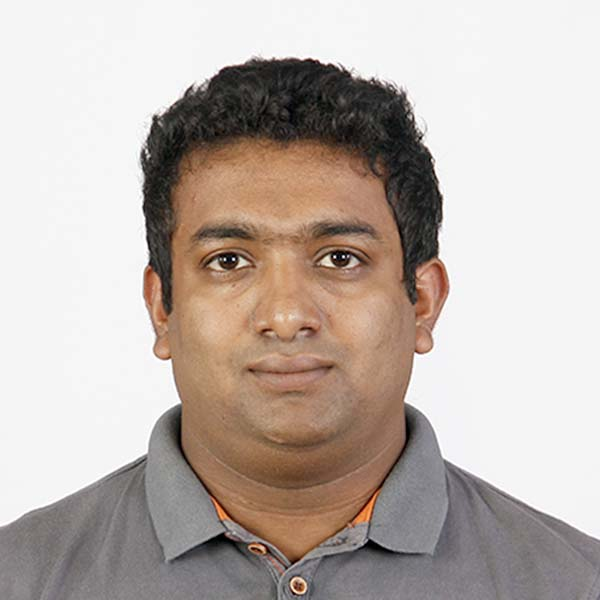
\includegraphics[scale=0.9]{img/photo.jpg}
    ~
  \header{Janitha}{Madushan}
      {Software Engineer}
   ~
  \section{Address}
    {\whitebodyfont No:04, "Sunhill,"\\
    Vajirapura,\\
    Nuwara-Eliya\\
    Sri-Lanka}
    ~
  \section{Phone}
    {\whitebodyfont +94 71 57 81 553\\
    +94 75 97 46 502}
    ~
  \section{Mail}
    \underline{\href{mailto:janithasen@gmail.com}{{\whitebodyfont janithasen@gmail.com}}}
    ~
  \section{Web}
  	\vspace{0.10cm}
    \underline{\href{https://www.linkedin.com/in/janithamadushan}{{\whitebodyfont linkedin}}}
    \\
	\vspace{0.10cm}
    \underline{\href{https://stackoverflow.com/story/jmadushan}{{\whitebodyfont stackoverflow}}}
	\\	
	\vspace{0.10cm}
    \underline{\href{https://github.com/janitham}{{\whitebodyfont github}}}
    ~
  \section{Langauges}
  	{\whitebodyfont Sinhaleese (Native)\\
    Engilsh}
    ~
  \section{Civil status}
    {\whitebodyfont Married}
  	~  
  \section{OS Preference}
    \asidelist{{\whitebodyfont Windows}}
    {\includegraphics[scale=0.30]{img/star.png}
    \includegraphics[scale=0.30]{img/star.png}
    \includegraphics[scale=0.30]{img/star.png}
    \includegraphics[scale=0.30]{img/star.png}
    \includegraphics[scale=0.30]{img/star.png}}
    \asidelist{\whitebodyfont{Linux}}
    {\includegraphics[scale=0.30]{img/star.png}
    \includegraphics[scale=0.30]{img/star.png}
    \includegraphics[scale=0.30]{img/star.png}
    \includegraphics[scale=0.30]{img/star_empty.png}
    \includegraphics[scale=0.30]{img/star_empty.png}}
    ~
  \section{Programming}
    \asidelist{{\whitebodyfont Java}}
    {\includegraphics[scale=0.30]{img/star.png}
    \includegraphics[scale=0.30]{img/star.png}
    \includegraphics[scale=0.30]{img/star.png}
    \includegraphics[scale=0.30]{img/star.png}
    \includegraphics[scale=0.30]{img/star_empty.png}}
    \asidelist{\whitebodyfont{C}}
    {\includegraphics[scale=0.30]{img/star.png}
    \includegraphics[scale=0.30]{img/star.png}
    \includegraphics[scale=0.30]{img/star.png}
    \includegraphics[scale=0.30]{img/star.png}
    \includegraphics[scale=0.30]{img/star_empty.png}}
    \asidelist{\whitebodyfont{Pyhon}}
    {\includegraphics[scale=0.30]{img/star.png}
    \includegraphics[scale=0.30]{img/star.png}
    \includegraphics[scale=0.30]{img/star.png}
    \includegraphics[scale=0.30]{img/star_empty.png}
    \includegraphics[scale=0.30]{img/star_empty.png}}
    \asidelist{\whitebodyfont{.NET}}
    {\includegraphics[scale=0.30]{img/star.png}
    \includegraphics[scale=0.30]{img/star.png}
    \includegraphics[scale=0.30]{img/star.png}
    \includegraphics[scale=0.30]{img/star_empty.png}
    \includegraphics[scale=0.30]{img/star_empty.png}}
    \asidelist{\whitebodyfont{PHP}}
    {\includegraphics[scale=0.30]{img/star.png}
    \includegraphics[scale=0.30]{img/star.png}
    \includegraphics[scale=0.30]{img/star.png}
    \includegraphics[scale=0.30]{img/star_empty.png}
    \includegraphics[scale=0.30]{img/star_empty.png}}
    ~
\end{aside}

\section{Experience}
\begin{entrylist}
  \entry
    {Nov. 15 - Now}
    {Software Developer}
    {Cambio Software Engineering}
    {I am working in automation team in configuration management team as a software developer. My responsibility 
    is to automate manual tasks in continuous delivery, continuous integration and management tools. On that tasks
    I developed various tools using various technologies. Mainly I developed tools using maven-plugins(MOJO), JAVA 
    and various devops technologies. Recently I am working in "Git Migration" sub project in "Tiger Infrastructure Project"\\}
  \entry
    {Oct. 15 - March. 16}
    {Internship}
    {IFS RD}
    {I worked with "Technology" team and two distinct internal projects during my internship. I developed one internal
	application and a research project. In that period I exposed to ASP.NET, ORACLE 11G/12C, PLSQL, ANDROID and JAVA.}
\end{entrylist}

\section{Education}
\begin{entrylist}
  \entry
    {Aug. 11 - June 15}
    {Bsc(Hons.) Computer Engineering}
    {Faculty of Engineering, University of Peradeniya}
    {I followed computer engineering at Faculty of engineering of University of peradeniya. There I specified in computer 		   	engineering also specified in software engineering}
\end{entrylist}

\newpage

\begin{aside}
  \vspace{1cm}
  \section{Places lived}
    \includegraphics[scale=0.62]{img/norway.png}
    ~
  \section{Languages}
    \asidelist{\textbf{Norwegian}}
    {\includegraphics[scale=0.30]{img/star.png}
    \includegraphics[scale=0.30]{img/star.png}
    \includegraphics[scale=0.30]{img/star.png}
    \includegraphics[scale=0.30]{img/star.png}
    \includegraphics[scale=0.30]{img/star.png}}
    \asidelist{\textbf{English}}
    {\includegraphics[scale=0.30]{img/star.png}
    \includegraphics[scale=0.30]{img/star.png}
    \includegraphics[scale=0.30]{img/star.png}
    \includegraphics[scale=0.30]{img/star.png}
    \includegraphics[scale=0.30]{img/star_empty.png}}
    \asidelist{\textbf{Faroese}}
    {\includegraphics[scale=0.30]{img/star.png}
    \includegraphics[scale=0.30]{img/star.png}
    \includegraphics[scale=0.30]{img/star_empty.png}
    \includegraphics[scale=0.30]{img/star_empty.png}
    \includegraphics[scale=0.30]{img/star_empty.png}}
    \asidelist{\textbf{German}}
    {\includegraphics[scale=0.30]{img/star.png}
    \includegraphics[scale=0.30]{img/star_empty.png}
    \includegraphics[scale=0.30]{img/star_empty.png}
    \includegraphics[scale=0.30]{img/star_empty.png}
    \includegraphics[scale=0.30]{img/star_empty.png}}
    ~
\end{aside}



\section{Projects}
\begin{entrylist}
  \entry
    {Oct. 16 - Now}
    {Brobet API \& Android app}
    {Project with Sondre Sallaup}
    {Spare time project with Sondre Sallaup, where I created and maintained
    the backend stack and native Android application.
    Backend stack consisted of a NodeJS (v6.x LTS) TypeScript GraphQL API with
    a PostgreSQL database using the ApolloStack libraries/toolset, ExpressJS http/ws server
    framework and Twitter Digits for authentication.
    \underline{Private repo}.\\}
  \entry
    {Aug. 15 - Oct. 15}
    {UiA Schedule for Android}
    {EnterCon project}
    {An Android application for displaying the schedule is a user-friendly,
    mobile-friendly manner. The scraping-logic from the C\# Schedule Scraper below
    was ported to Java so that the app runs natively.
    \underline{\href{https://github.com/EnterCon/UiA-Timeplan-Android}
    {Github repository}}.\\}
  \entry
    {June 15}
    {UiA Schedule Scraper}
    {Solo project}
    {A C\# console application scraping university programme schedule information
    of their webpage, outputting JSON.
    \underline{\href{https://github.com/EnterCon/UiA-ScheduleScraper}
    {Github repository}}.\\}
\end{entrylist}


\section{Certifications}
\begin{entrylist}
  \entry
    {Oct. 15}
    {PRINCE2 Foundation certification}
    {University of Agder, Kristiansand}
    {Foundation-level Project Management certification.}
\end{entrylist}

\vspace{1.5cm}
\begin{flushright}
\emph{Martin Othamar}
\end{flushright}
\begin{flushright}
\emph{\today}
\end{flushright}

\end{document}
